% !TeX program = xelatex
% UTF-8; compile with XeLaTeX twice.
\documentclass[UTF8,fontset=fandol,a4paper,11pt]{ctexart}
\usepackage[margin=2.35cm,headheight=14pt]{geometry}
\usepackage{amsmath,amssymb,bm,booktabs,tabularx,array}
\usepackage{graphicx,float,caption,enumitem,xcolor,fancyhdr}
\usepackage[numbers,sort&compress]{natbib}
\usepackage{hyperref,xurl,microtype}
\usepackage[section]{placeins}
\definecolor{navy}{HTML}{17324D}
\definecolor{teal}{HTML}{287D8E}
\hypersetup{colorlinks=true,linkcolor=navy,citecolor=teal,urlcolor=teal,
 pdftitle={Auto-ORCA: LLM-Guided Autonomous Exploration of Potential Energy Surfaces Using DFT},
 pdfauthor={Auto-ORCA}}
\urlstyle{same}
\graphicspath{{figures/}}
\renewcommand{\arraystretch}{1.18}
\setlength{\tabcolsep}{5pt}
\setlength{\emergencystretch}{3em}
\linespread{1.12}
\renewcommand{\topfraction}{0.9}
\renewcommand{\bottomfraction}{0.85}
\renewcommand{\textfraction}{0.08}
\renewcommand{\floatpagefraction}{0.8}
\setlist{nosep,leftmargin=2em}
\captionsetup{font=small,labelfont=bf,labelsep=quad}
\ctexset{section={format=\Large\bfseries},subsection={format=\large\bfseries}}
\pagestyle{fancy}
\fancyhf{}
\fancyhead[L]{\small Auto-ORCA}
\fancyhead[R]{\small LLM 引导的自主量子化学计算}
\fancyfoot[C]{\thepage}
\newcolumntype{Y}{>{\raggedright\arraybackslash}X}
\newcommand{\Eh}{E_{\mathrm h}}
\newcommand{\code}[1]{\texttt{#1}}
\title{\vspace{-1.3cm}\bfseries Auto-ORCA:\\[0.3em]
 \Large LLM-Guided Autonomous Exploration of\\
 Potential Energy Surfaces Using DFT\\[0.6em]
 \large 大语言模型引导的 DFT 势能面自主探索}
\author{}
\date{}
\begin{document}
\maketitle
\vspace{-1.6cm}
\begin{abstract}
分子势能面探索需要在结构准备、电子结构计算、收敛判断与后续采样之间反复作出决策，固定脚本难以直接适应开放的科学需求。本文提出 Auto-ORCA，将大语言模型的任务规划与代码生成能力连接至受管理的 ORCA 执行环境。系统采用单一决策循环，将科学目标与可修订计划分离，通过通用工具校验并执行生成的 Python 和 ORCA 输入，再依据真实输出组织后续行动。测试覆盖乙醇结构优化与振动频率、正己烷候选构象能量、正丁烷二面角扫描、丙酮垂直激发、乙醇环境电子能量差、HCN 核磁屏蔽及甲醛极化率七个问题。按 ORCA 计算正常完成并产生数值结果的口径，六项标记为成功，计算成功率为 $6/7=85.7\%$。乙醇优化收敛并获得 21 个正频率、0 个虚频；正己烷完成六个候选几何的单点能量比较；丙酮获得五个单重态激发能；两种基组下 CPCM 水环境相对气相的电子能量差分别为 $-18.276507$ 和 $-16.607972$ kJ mol$^{-1}$；HCN 获得三核完整屏蔽张量。正丁烷六个约束优化点计算成功，但实际二面角仍待独立核查；甲醛尚无极化率数值。结果支持通用工具与生成代码组合执行多类 DFT 任务的可行性，完整势能面结论仍需进一步的几何验证与采样证据。
\end{abstract}
\noindent\textbf{关键词：}Auto-ORCA；大语言模型；密度泛函理论；势能面；代码生成；自主量子化学

\section{引言}
分子结构、构象稳定性和反应路径与势能面紧密相关。密度泛函理论（density functional theory, DFT）通过电子密度描述多电子体系，Kohn--Sham 框架为实际电子结构求解提供了基础\cite{hk,ks}。然而，单次求解只回答特定方法、几何与环境下的问题。势能面研究还需要组织结构优化、振动分析、候选比较及约束扫描，并根据中间结果决定下一步计算。

ASE、AiiDA、Atomate2 与 cclib 分别提供原子模拟接口、来源追踪、计算流程组合及输出解析能力\cite{ase,aiida,atomate2,cclib}。这些工具使已知协议能够可靠复用，但新的科学问题仍可能需要专门编写采样与分析程序。大语言模型为连接自然语言目标与可执行操作提供了另一条路径。ReAct、Toolformer 和 Reflexion 探索了推理、工具使用与反馈修正\cite{react,toolformer,reflexion}；ChemCrow 与 Coscientist 则展示了语言模型组织化学工具和研究操作的可行性\cite{chemcrow,coscientist}。

自主电子结构计算的核心挑战是维持科学目标与实际证据之间的一致性。AutoDFT 强调将执行结果反馈至后续规划\cite{autodft}。Lee 与 Rondinelli 对自主多参考量子化学计算的研究进一步将 Agent 架构、计算方法与结果评价分别展开，并强调数值收敛与电子态身份之间的区别\cite{multirefagent}。本文借鉴这种问题导向的组织方式，研究 DFT 任务中代码生成、实际执行和结果解释的连接。

本文提出 Auto-ORCA，其完整名称为 \emph{LLM-Guided Autonomous Exploration of Potential Energy Surfaces Using DFT}。系统基于 ORCA 与 ORCA Python Interface（OPI）\cite{orca2020,orca6,opipaper}，通过单一 Agent 决策循环组合固定通用工具与现场生成代码。本文关注三个问题：生成代码能否表达多种分子计算任务，统一执行入口能否获得真实数值，以及这些数值能够支持何种科学结论。结构优化、构象比较与二面角扫描构成势能面相关测试，激发态、环境效应与响应张量用于检验性质计算的扩展能力。

\section{Agent 架构}
\subsection{单一决策循环与任务代码生成}
Auto-ORCA 将自然语言需求转化为科学目标、计算条件与可执行计划。模型根据当前证据提出参数、Python 程序或 ORCA 输入；程序检查依赖、权限与资源后执行；新结果接受读取、检查与目标评价，并反馈至下一轮决策。图 \ref{fig:architecture} 给出总体结构。成功计算与失败信息均进入反馈，系统不预设优化、频率和单点的固定执行顺序。

\begin{figure}[htbp]
\centering
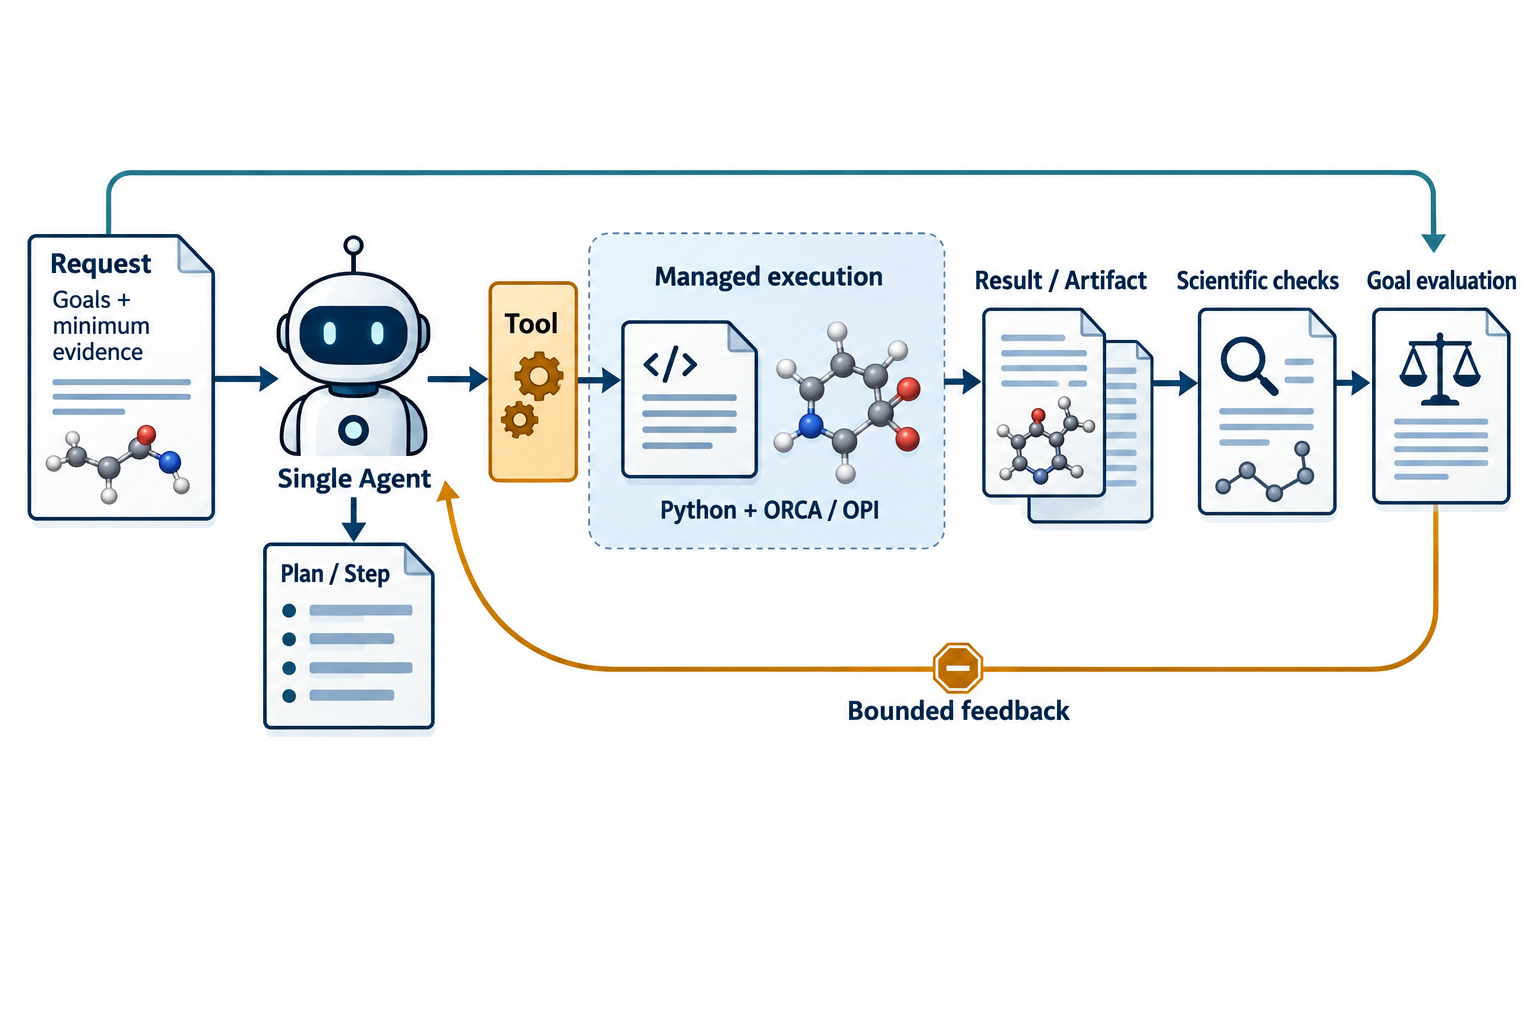
\includegraphics[width=\linewidth,trim=14 205 14 112,clip]{method-overview.png}
\caption{Auto-ORCA 的单一决策循环。原始目标与最低证据要求约束结果评价；模型通过通用工具组织受管理的 Python 与 ORCA 执行，并依据返回证据调整计划。}
\label{fig:architecture}
\end{figure}

任务特定算法由生成代码表达，通用工具负责输入校验、执行与产物管理。例如，程序可构建有限几何集合、逐一请求能量计算，再按统一单位比较结果。OPI 输入、原生 ORCA 输入和 Python 内部计算请求复用同一执行入口\cite{opi}；薄接口返回计算回执与原始产物，不封装针对单个问题的隐式求解算法。该设计使同一组工具能够处理不同任务，同时保留明确的执行边界。

\subsection{目标保持与证据管理}
系统使用 Request、Plan、Step、Tool、Run、Result 和 Artifact 表达需求、路线、操作、执行接口、运行记录、结果与原始产物。科学目标及最低证据要求独立于 Plan 保存，计划修改只改变实现路线。例如，在同一几何上比较气相与水环境能量，不能被无说明地改成两次独立优化；修复代码也不能通过删除目标获得形式上的完成。

模型负责提出动作和修复建议，程序负责判定动作是否可执行以及输出是否满足规定检查。初始几何、输入、生成程序与各次原始输出独立保存，通过内容校验绑定来源。读取证据不隐式触发计算或转换，额外分析作为明确操作执行。对于尚未纳入标准检查的性质，可保存带来源、单位和限制说明的观察，模型或任务脚本不能自行授予科学资格。

\subsection{反馈、资源与停止}
反馈保留原始目标、当前结果和有效诊断，并提供可查询的证据来源。错误信息用于定位输入、程序或求解失败；成功输出用于判断是否需要补充几何检查、采样或跨结果分析。执行状态不明时先核对已有事实，避免重复启动。

资源约束覆盖生成程序及其内部 ORCA 子计算。令预算维度 $k$ 的上限为 $B_k$、累计用量为 $U_k$、新动作预留为 $r_k$，执行前要求
\begin{equation}
U_k+r_k\leq B_k.
\end{equation}
内部计算、代码重试和模型纠错均计入累计用量，暂停或恢复不重置消耗。生成代码仅在受管理的任务环境中访问输入副本、必要运行库与任务产物目录。停止后保留已经完成的计算结果及尚未回答的问题。

\section{计算方法与评价}
\subsection{计算设置与科学任务}
计算使用 ORCA 6.1.1，并通过 OPI 2.0.0 及统一执行接口组织。所用本地资源为 4 核、计算进程树内存上限 1024 MiB、ORCA MaxCore 192 MiB/进程，环境计算并发为 1。MaxCore 为 ORCA 内部内存参数，与进程树总内存限制分别设置。

七个测试问题的实际方法见表 \ref{tab:task-overview}，已完成计算的体系均为中性单重态。r$^{2}$SCAN-3c 采用其内置 def2-mTZVPP 基组\cite{r2scan3c}；其他方法与基组按实际计算逐项报告，基组体系遵循 def2 定义\cite{def2}。垂直激发采用完整线性响应 TDDFT\cite{tddft}，水环境使用 CPCM 连续介质描述\cite{cpcm}。除明确说明的结构优化与约束优化外，各项结果均对应指定的固定几何。

\subsection{计算成功率与结果解释}
以 ORCA 原始输出的正常结束记录作为计算完成依据。对本文所列每个问题，只要已有相应 ORCA 计算正常完成并保存数值结果，即标记为\textbf{成功}；尚无实际数值结果则标记为\textbf{未完成}。因此，T3 的六个已完成计算点计为成功，其未计算端点与角度核查限制在结果中明确说明。
\begin{equation}
R_{\mathrm{calc}}=\frac{N_{\mathrm{success}}}{N_{\mathrm{questions}}}
=\frac{6}{7}\approx85.7\%.
\label{eq:success-rate}
\end{equation}
该比例以七个问题为分母，每题计数一次。科学结论根据实际收敛、几何、方法和性质证据分别解释：正常结束不单独证明全局最低构象、正确的扫描势垒或实验可比的响应量。

相对电子能量以指定候选集合内的参考值为零。能量换算使用 $1\,\Eh=2625.4996394799$ kJ mol$^{-1}$；电子能、振动频率、激发能与屏蔽张量保留原始输出或核查记录的精度。原始数据与来源记录用于复核和复用\cite{fair}。本报告呈现已有计算结果，不将所列成功率解释为任意新任务的成功概率，也不以缺少独立参考的能量差评价方法准确度。

\section{结果与讨论}
% !TeX root = main.tex
\subsection{七个问题的结果概览}
以下七个科学问题用于测试 Auto-ORCA Agent 的任务组织与执行能力，能力定位见表 \ref{tab:agent-capability-design}。表 \ref{tab:task-overview} 汇总各题的实际方法与结果。T1--T5 和 H1 标记为成功，H2 未完成，计算成功率为 $6/7=85.7\%$。各项数值与科学解释如下。

\begin{table}[H]
\centering\small
\caption{七个测试问题的实际计算方法与结果。成功表示已有 ORCA 计算正常完成并产生相应数值。}
\label{tab:task-overview}
\begin{tabularx}{\linewidth}{l>{\raggedright\arraybackslash}p{2.5cm}>{\raggedright\arraybackslash}p{3.3cm}>{\raggedright\arraybackslash}p{1.15cm}Y}
\toprule
编号 & 问题 & 实际方法 & 状态 & 主要结果\\
\midrule
T1 & 乙醇优化与频率 & r$^{2}$SCAN-3c & 成功 & 优化收敛；21 个正频率，0 个虚频\\
T2 & 正己烷候选能量 & r$^{2}$SCAN-3c 单点 & 成功 & 6 个候选几何的能量排序\\
T3 & 正丁烷二面角扫描 & r$^{2}$SCAN-3c 约束优化 & 成功 & 6 个收敛点；实际角度待核查\\
T4 & 丙酮垂直激发 & PBE0/def2-SVP，LR-TDDFT & 成功 & 5 个单重态激发能及振子强度\\
T5 & 乙醇环境能量差 & B3LYP/def2-TZVP 与 def2-SVP & 成功 & 两种基组下的气相与 CPCM 水电子能差\\
H1 & HCN 核磁屏蔽 & PBE0/def2-TZVP，GIAO & 成功 & C、N、H 三核完整屏蔽张量\\
H2 & 甲醛极化率及旋转一致性 & 尚无实际计算结果 & 未完成 & 未获得极化率数值\\
\bottomrule
\end{tabularx}
\end{table}

\subsection{T1：乙醇结构优化与振动频率}
\paragraph{问题}
优化乙醇结构，并通过振动频率判断所得结构是否为局部极小值。

\paragraph{方法}
采用 r$^{2}$SCAN-3c 及其内置 def2-mTZVPP 基组，在气相、中性单重态条件下进行结构优化与振动频率计算。

\paragraph{结果}
\textbf{计算成功。}几何优化已收敛，优化后电子能量为 $-155.002345492244\,\Eh$。获得 21 个正振动频率、6 个投影后的平动与转动零频以及 0 个虚频。全部正频率见表 \ref{tab:t1-frequencies}。这些结果支持该方法下的局部极小值结构，不能证明全局最低能构象；优化后坐标保存在相应 ORCA 输出的 XYZ 文件中。

\begin{table}[H]
\centering\small
\caption{乙醇的 21 个正振动频率，单位 cm$^{-1}$。}
\label{tab:t1-frequencies}
\begin{tabular}{rrrrrrr}
\toprule
270.90 & 298.95 & 425.86 & 811.51 & 882.13 & 1052.13 & 1066.45\\
1134.41 & 1282.25 & 1371.13 & 1396.18 & 1418.25 & 1483.33 & 1487.57\\
1509.53 & 2969.59 & 3004.65 & 3061.83 & 3088.36 & 3105.66 & 3819.31\\
\bottomrule
\end{tabular}
\end{table}

\subsection{T2：正己烷候选构象的单点电子能量}
\paragraph{问题}
比较正己烷候选几何的电子能量，确定所计算集合内的相对能量顺序。

\paragraph{方法}
采用 r$^{2}$SCAN-3c，在气相、中性单重态条件下，对保存的六个候选几何分别进行单点计算。相对能量以 cand\_05 为零。

\paragraph{结果}
\textbf{计算成功。}六个候选均获得电子能量，结果见表 \ref{tab:t2-energies}。cand\_05 在该集合中能量最低，cand\_03 相对高出 12.608656 kJ mol$^{-1}$。这些是候选几何上的单点结果，不能表述为六个构象均经过 DFT 优化，也不能据此推断全局最低构象或自由能排序。

\begin{table}[H]
\centering\small
\caption{正己烷六个候选几何的单点电子能量。}
\label{tab:t2-energies}
\begin{tabular}{lrr}
\toprule
候选 & 电子能量 / $\Eh$ & 相对能量 / kJ mol$^{-1}$\\
\midrule
cand\_05 & $-236.992066202851$ & 0.000000\\
cand\_04 & $-236.991445556657$ & 1.629506\\
cand\_01 & $-236.991444090308$ & 1.633356\\
cand\_00 & $-236.991421448668$ & 1.692802\\
cand\_06 & $-236.991245997872$ & 2.153448\\
cand\_03 & $-236.987263819406$ & 12.608656\\
\bottomrule
\end{tabular}
\end{table}

\subsection{T3：正丁烷二面角扫描}
\paragraph{问题}
通过约束优化获得正丁烷不同目标二面角下的电子能量，考察扭转势能变化。

\paragraph{方法}
主要计算采用 r$^{2}$SCAN-3c、气相、中性单重态条件，在指定目标二面角下进行约束优化。另列一个 B3LYP/def2-TZVP 计算点，单独报告其几何核查结果。

\paragraph{结果}
\textbf{计算成功。}r$^{2}$SCAN-3c 的六个计算点均有 ORCA 正常结束及优化收敛记录，结果见表 \ref{tab:t3-energies}；$+180^\circ$ 点未启动。表中第一列仅为输入目标角度标签。生成脚本报告的实际角度与输入标签存在矛盾，尚未通过独立几何核查确认。因此，能量为真实计算产出，但标签不能直接视为已经验证的实际二面角，也不能据此确认扫描势垒；尤其不能直接将 $+120^\circ$ 的高能量解释为可信的物理势垒。

\begin{table}[H]
\centering\small
\caption{正丁烷六个约束优化点。角度为输入目标标签；相对能量为已保存数值。}
\label{tab:t3-energies}
\begin{tabular}{rrr}
\toprule
输入目标角度 / $^\circ$ & 电子能量 / $\Eh$ & 相对能量 / kJ mol$^{-1}$\\
\midrule
$-180$ & $-158.392470368263$ & 0.000000\\
$-120$ & $-158.387146187943$ & 13.978634\\
$-60$ & $-158.391526560891$ & 2.477966\\
$0$ & $-158.383528626170$ & 23.476541\\
$+60$ & $-158.391526702130$ & 2.477595\\
$+120$ & $-158.358972460497$ & 87.948745\\
\bottomrule
\end{tabular}
\end{table}

B3LYP/def2-TZVP 计算点的输入目标角度为 $-180^\circ$。独立几何核查得到实际角度 $179.999995786^\circ$，按周期意义符合目标；收敛电子能量为 $-158.397118300397\,\Eh$。该点采用不同方法，不并入表 \ref{tab:t3-energies} 的相对能量。

\subsection{T4：丙酮前五个单重态垂直激发}
\paragraph{问题}
获得丙酮前五个单重态垂直激发的激发能、波长和振子强度。

\paragraph{方法}
在固定准备几何上采用 PBE0/def2-SVP、气相、中性单重态，通过完整线性响应 TDDFT（LR-TDDFT，\code{TDA=false}）求解五个单重激发态。振子强度取 ORCA 的长度规范输出。

\paragraph{结果}
\textbf{计算成功。}SCF 和响应求解均有收敛记录，五个激发态的数值见表 \ref{tab:t4-excitations}。最低单重态垂直激发能为 4.197061 eV，对应波长 295.4 nm。

\begin{table}[H]
\centering\small
\caption{丙酮前五个单重态垂直激发。振子强度 $f$ 为无量纲。}
\label{tab:t4-excitations}
\begin{tabular}{crrr}
\toprule
激发态 & 激发能 / eV & 波长 / nm & 振子强度 $f$\\
\midrule
$S_{1}$ & 4.197061 & 295.4 & 0.000007493\\
$S_{2}$ & 7.464499 & 166.1 & 0.023781213\\
$S_{3}$ & 8.406988 & 147.5 & 0.001899769\\
$S_{4}$ & 8.572306 & 144.6 & 0.060276158\\
$S_{5}$ & 8.640904 & 143.5 & 0.004121254\\
\bottomrule
\end{tabular}
\end{table}

\subsection{T5：乙醇气相与 CPCM 水环境的电子能量差}
\paragraph{问题}
比较相同几何下乙醇在气相与 CPCM 水环境中的电子能量。

\paragraph{方法}
采用 B3LYP、中性单重态，分别使用 def2-TZVP 与 def2-SVP 基组。每种基组下的气相与水环境计算使用同一份初始几何；该几何不是 T1 的优化后结构。定义 $\Delta E=E_{\mathrm{water}}-E_{\mathrm{gas}}$。

\paragraph{结果}
\textbf{计算成功。}每种基组均完成气相与 CPCM 水环境的两次 ORCA 计算。表 \ref{tab:t5-energies} 给出电子能量，表 \ref{tab:t5-differences} 给出差值。负号表示相应模型和固定几何下水环境电子能量低于气相。这里得到的是\textbf{电子能量差，不是水合自由能}。

\begin{table}[H]
\centering\small
\caption{乙醇在气相与 CPCM 水环境中的电子能量。}
\label{tab:t5-energies}
\begin{tabular}{lrr}
\toprule
基组 & 气相电子能量 / $\Eh$ & CPCM 水电子能量 / $\Eh$\\
\midrule
def2-TZVP & $-155.002778990957$ & $-155.009740144896$\\
def2-SVP & $-154.817054999208$ & $-154.823380641772$\\
\bottomrule
\end{tabular}
\end{table}

\begin{table}[H]
\centering\small
\caption{乙醇水环境相对气相的电子能量差。}
\label{tab:t5-differences}
\begin{tabular}{lrr}
\toprule
基组 & $\Delta E$ / $\Eh$ & $\Delta E$ / kJ mol$^{-1}$\\
\midrule
def2-TZVP & $-0.006961153939$ & $-18.276507$\\
def2-SVP & $-0.006325642564$ & $-16.607972$\\
\bottomrule
\end{tabular}
\end{table}

\subsection{H1：HCN 的 GIAO 核磁屏蔽张量}
\paragraph{问题}
获得 HCN 各原子的核磁屏蔽张量及各向同性屏蔽值。

\paragraph{方法}
在固定初始几何上采用 PBE0/def2-TZVP、气相、中性单重态和 GIAO 方法。原子顺序为 C$_0$、N$_1$、H$_2$。

\paragraph{结果}
\textbf{计算成功。}总电子能量为 $-93.345070922944\,\Eh$。ORCA 打印的各向同性屏蔽见表 \ref{tab:h1-isotropic}；完整总屏蔽张量见式 \eqref{eq:h1-tensors}，单位为 ppm，行列顺序均为 X、Y、Z，保留原始输出的三位小数。

\begin{table}[H]
\centering\small
\caption{HCN 的各向同性核磁屏蔽。}
\label{tab:h1-isotropic}
\begin{tabular}{cr}
\toprule
原子 & 各向同性屏蔽 / ppm\\
\midrule
C$_0$ & 79.051\\
N$_1$ & $-34.068$\\
H$_2$ & 29.850\\
\bottomrule
\end{tabular}
\end{table}

\begin{equation}
\begin{aligned}
\bm{\sigma}_{\mathrm{C}_0}&=\begin{pmatrix}
279.306 & -0.724 & -0.000 \\
-1.638 & -21.077 & 0.000 \\
-0.000 & 0.000 & -21.076
\end{pmatrix},\\[0.8em]
\bm{\sigma}_{\mathrm{N}_1}&=\begin{pmatrix}
340.398 & -1.842 & -0.000 \\
-0.044 & -221.291 & 0.000 \\
0.000 & 0.000 & -221.309
\end{pmatrix},\\[0.8em]
\bm{\sigma}_{\mathrm{H}_2}&=\begin{pmatrix}
39.712 & 0.055 & -0.000 \\
-0.114 & 24.919 & -0.000 \\
-0.000 & -0.000 & 24.920
\end{pmatrix}.
\end{aligned}
\label{eq:h1-tensors}
\end{equation}
各向同性屏蔽为张量迹的三分之一；表中数值直接采用 ORCA 打印的摘要，不由已舍入的矩阵重新计算。上述量未通过参考物换算，不能直接称为实验化学位移。H$_2$ 表示氢原子索引，与下节的 H2 任务编号无关。

\subsection{H2：甲醛静态极化率及旋转一致性}
\paragraph{问题}
获得甲醛两个取向下的静态极化率张量与各向同性极化率，并比较旋转前后的物理一致性。

\paragraph{方法}
已准备几何与旋转方案，拟分别求取两个取向的极化率并进行坐标变换比较。

\paragraph{结果}
\textbf{未完成。}目前没有实际 ORCA 极化率数值，两个取向的极化率张量、各向同性极化率及旋转一致性比较均未得到。准备好的几何和旋转方案不计为计算结果。


\subsection{跨任务表现与结果边界}
六项成功结果覆盖结构优化、谐振频率、单点能量、约束优化、垂直激发、环境能量比较及核磁屏蔽，说明生成程序可以围绕共同 ORCA 入口组织不同类型的计算。图 \ref{fig:current-results} 以正己烷候选能量和丙酮激发响应展示两个结果实例。

\begin{figure}[htbp]
\centering
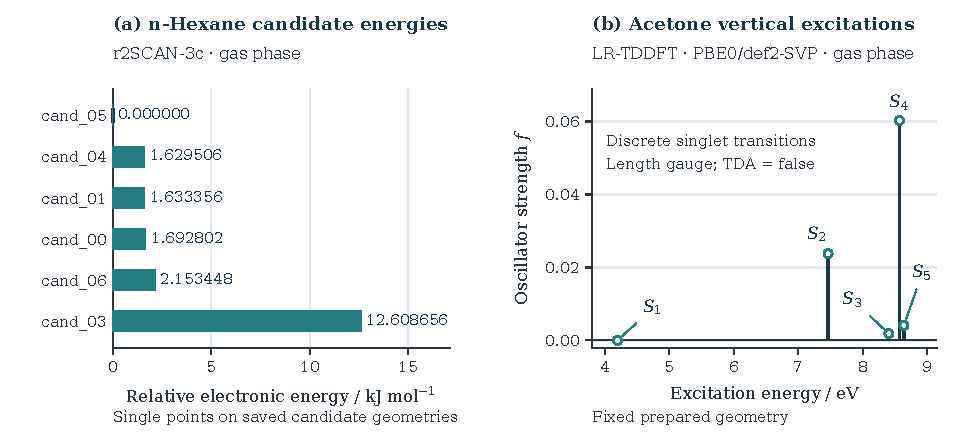
\includegraphics[width=\linewidth]{current-results.pdf}
\caption{数值结果的两个实例。（a）正己烷六个候选几何的 r$^{2}$SCAN-3c 单点相对电子能，以 cand\_05 为零。（b）丙酮 PBE0/def2-SVP 完整 LR-TDDFT 的离散垂直激发及长度规范振子强度。右图不含谱线展宽；两图均对应各自指定的固定几何。}
\label{fig:current-results}
\end{figure}

与势能面直接相关的结果具有不同证据范围：T1 的收敛优化和无虚频支持局部极小值；T2 给出有限候选几何上的单点排序；T3 保存了六个收敛约束优化点，但缺少经过独立确认的角度对应。因此，现有结果支持势能面相关操作的执行能力，尚不能据此宣称完成全局势能面搜索或获得可信的完整扭转势垒。

性质计算同样需要明确物理量含义。T4 对应固定准备几何上的垂直激发，T5 给出固定几何下的电子能量差，H1 给出绝对核磁屏蔽。H2 尚无张量数值，不能开展旋转一致性验证。后续验证应优先补齐这些具体缺口，并采用相同条件下的重复计算及独立参考评价可重复性和准确度。

\section{结论}
本文提出 Auto-ORCA，以单一 Agent 决策循环组合通用工具与生成代码，通过统一 ORCA 入口执行 DFT 任务，并分别保存原始目标、实际条件和数值证据。七个测试问题中，T1--T5 与 H1 已完成 ORCA 计算并取得结果，按本文定义的计算成功口径，成功率为 $6/7=85.7\%$；H2 尚无实际极化率数值。

主要结果包括乙醇的收敛优化结构与 21 个正频率、正己烷六个候选的单点能量、正丁烷六个约束优化点、丙酮五个单重态激发、两种基组下的气相与水环境电子能量差，以及 HCN 三核完整屏蔽张量。结构与性质的解释仍取决于各自证据：局部极小值不等于全局最优，正丁烷角度对应尚待核查，环境电子能量差不等于水合自由能。未来工作应围绕几何确认、采样完整性、响应张量验证和重复试验，进一步检验自主势能面探索的可靠性。

\paragraph{数据与材料可用性}
本文数值来自已保存的 ORCA 原始输出及对应核查记录。LaTeX 源文件、结构化数值、来源校验信息与绘图程序随报告提供；本次文档修订未启动新的 ORCA 或模型计算。架构示意图由 GPT Image 辅助绘制，数值图直接依据所列结果生成。

\medskip
\renewcommand{\refname}{参考文献}
\begingroup
\footnotesize
\linespread{1.05}\selectfont
\interlinepenalty=10000
% References cited by the current Auto-ORCA manuscript.
\begin{thebibliography}{99}
\setlength{\itemsep}{0.25em}

\bibitem{hk}
P. Hohenberg and W. Kohn.
Inhomogeneous Electron Gas.
\emph{Physical Review} \textbf{136}, B864--B871 (1964).
\href{https://doi.org/10.1103/PhysRev.136.B864}{doi:10.1103/PhysRev.136.B864}.

\bibitem{ks}
W. Kohn and L. J. Sham.
Self-Consistent Equations Including Exchange and Correlation Effects.
\emph{Physical Review} \textbf{140}, A1133--A1138 (1965).
\href{https://doi.org/10.1103/PhysRev.140.A1133}{doi:10.1103/PhysRev.140.A1133}.

\bibitem{orca2020}
F. Neese, F. Wennmohs, U. Becker, et al.
The ORCA quantum chemistry program package.
\emph{The Journal of Chemical Physics} \textbf{152}, 224108 (2020).
\href{https://doi.org/10.1063/5.0004608}{doi:10.1063/5.0004608}.

\bibitem{orca6}
F. Neese.
Software Update: The ORCA Program System---Version 6.0.
\emph{WIREs Computational Molecular Science} \textbf{15}, e70019 (2025).
\href{https://doi.org/10.1002/wcms.70019}{doi:10.1002/wcms.70019}.

\bibitem{opipaper}
T. Tetenberg, H. Neugebauer, C. Plett, et al.
ORCA Meets Python---The ORCA Python Interface OPI.
\emph{Journal of Chemical Theory and Computation} \textbf{22}, 4951--4967 (2026).
\href{https://doi.org/10.1021/acs.jctc.5c02141}{doi:10.1021/acs.jctc.5c02141}.

\bibitem{ase}
A. H. Larsen, J. J. Mortensen, J. Blomqvist, et al.
The atomic simulation environment---a Python library for working with atoms.
\emph{Journal of Physics: Condensed Matter} \textbf{29}, 273002 (2017).
\href{https://doi.org/10.1088/1361-648X/aa680e}{doi:10.1088/1361-648X/aa680e}.

\bibitem{aiida}
G. Pizzi, A. Cepellotti, R. Sabatini, et al.
AiiDA: automated interactive infrastructure and database for computational science.
\emph{Computational Materials Science} \textbf{111}, 218--230 (2016).
\href{https://doi.org/10.1016/j.commatsci.2015.09.013}{doi:10.1016/j.commatsci.2015.09.013}.

\bibitem{atomate2}
A. M. Ganose, H. Sahasrabuddhe, M. Asta, et al.
Atomate2: modular workflows for materials science.
\emph{Digital Discovery} \textbf{4}, 1944--1973 (2025).
\href{https://doi.org/10.1039/D5DD00019J}{doi:10.1039/D5DD00019J}.

\bibitem{cclib}
N. M. O'Boyle, A. L. Tenderholt, and K. M. Langner.
cclib: A library for package-independent computational chemistry algorithms.
\emph{Journal of Computational Chemistry} \textbf{29}, 839--845 (2008).
\href{https://doi.org/10.1002/jcc.20823}{doi:10.1002/jcc.20823}.

\bibitem{react}
S. Yao, J. Zhao, D. Yu, et al.
ReAct: Synergizing Reasoning and Acting in Language Models.
\emph{The Eleventh International Conference on Learning Representations (ICLR)} (2023).
\href{https://openreview.net/forum?id=WE_vluYUL-X}{OpenReview: WE\_vluYUL-X};
\href{https://doi.org/10.48550/arXiv.2210.03629}{预印本 doi:10.48550/arXiv.2210.03629}.

\bibitem{toolformer}
T. Schick, J. Dwivedi-Yu, R. Dessì, et al.
Toolformer: Language Models Can Teach Themselves to Use Tools.
\emph{Advances in Neural Information Processing Systems} \textbf{36}, 68539--68551 (2023).
\href{https://doi.org/10.52202/075280-2997}{doi:10.52202/075280-2997}.

\bibitem{reflexion}
N. Shinn, F. Cassano, A. Gopinath, et al.
Reflexion: Language Agents with Verbal Reinforcement Learning.
\emph{Advances in Neural Information Processing Systems} \textbf{36}, 8634--8652 (2023).
\href{https://doi.org/10.52202/075280-0377}{doi:10.52202/075280-0377}.

\bibitem{chemcrow}
A. M. Bran, S. Cox, O. Schilter, et al.
Augmenting large language models with chemistry tools.
\emph{Nature Machine Intelligence} \textbf{6}, 525--535 (2024).
\href{https://doi.org/10.1038/s42256-024-00832-8}{doi:10.1038/s42256-024-00832-8}.

\bibitem{coscientist}
D. A. Boiko, R. MacKnight, B. Kline, et al.
Autonomous chemical research with large language models.
\emph{Nature} \textbf{624}, 570--578 (2023).
\href{https://doi.org/10.1038/s41586-023-06792-0}{doi:10.1038/s41586-023-06792-0}.

\bibitem{autodft}
P. Yang, Z. Zhang, Y. Li, et al.
AutoDFT: A Closed-Loop Multi-Agent Framework for Autonomous DFT Calculations.
\emph{arXiv preprint}, arXiv:2605.26179v2 (2026), 2026年6月4日版本.
\href{https://doi.org/10.48550/arXiv.2605.26179}{doi:10.48550/arXiv.2605.26179}.

\bibitem{multirefagent}
V. C. Lee and J. M. Rondinelli.
Can Autonomous LLM Agents Execute Multireference Quantum Chemistry Calculations?
\emph{arXiv preprint}, arXiv:2609.13357v1 (2026), 2026年9月11日版本.
\href{https://doi.org/10.48550/arXiv.2609.13357}{doi:10.48550/arXiv.2609.13357}.

\bibitem{fair}
M. D. Wilkinson, M. Dumontier, I. J. Aalbersberg, et al.
The FAIR Guiding Principles for scientific data management and stewardship.
\emph{Scientific Data} \textbf{3}, 160018 (2016).
\href{https://doi.org/10.1038/sdata.2016.18}{doi:10.1038/sdata.2016.18}.

\bibitem{gfn2}
C. Bannwarth, S. Ehlert, and S. Grimme.
GFN2-xTB---An Accurate and Broadly Parametrized Self-Consistent Tight-Binding Quantum Chemical Method with Multipole Electrostatics and Density-Dependent Dispersion Contributions.
\emph{Journal of Chemical Theory and Computation} \textbf{15}, 1652--1671 (2019).
\href{https://doi.org/10.1021/acs.jctc.8b01176}{doi:10.1021/acs.jctc.8b01176}.

\bibitem{crest}
P. Pracht, F. Bohle, and S. Grimme.
Automated exploration of the low-energy chemical space with fast quantum chemical methods.
\emph{Physical Chemistry Chemical Physics} \textbf{22}, 7169--7192 (2020).
\href{https://doi.org/10.1039/C9CP06869D}{doi:10.1039/C9CP06869D}.

\bibitem{cpcm}
M. Cossi, N. Rega, G. Scalmani, et al.
Energies, structures, and electronic properties of molecules in solution with the C-PCM solvation model.
\emph{Journal of Computational Chemistry} \textbf{24}, 669--681 (2003).
\href{https://doi.org/10.1002/jcc.10189}{doi:10.1002/jcc.10189}.

\bibitem{tddft}
E. Runge and E. K. U. Gross.
Density-Functional Theory for Time-Dependent Systems.
\emph{Physical Review Letters} \textbf{52}, 997--1000 (1984).
\href{https://doi.org/10.1103/PhysRevLett.52.997}{doi:10.1103/PhysRevLett.52.997}.

\bibitem{opi}
FACCTs.
\emph{ORCA Python Interface (OPI) 2.0 Documentation}.
官方技术文档，访问日期：2026年10月21日.
\url{https://www.faccts.de/docs/opi/2.0/docs/}.

\bibitem{r2scan3c}
S. Grimme, A. Hansen, S. Ehlert, and J.-M. Mewes.
r$^{2}$SCAN-3c: A "Swiss army knife" composite electronic-structure method.
\emph{The Journal of Chemical Physics} \textbf{154}, 064103 (2021).
\href{https://doi.org/10.1063/5.0040021}{doi:10.1063/5.0040021}.

\bibitem{def2}
F. Weigend and R. Ahlrichs.
Balanced basis sets of split valence, triple zeta valence and quadruple zeta valence quality for H to Rn: Design and assessment of accuracy.
\emph{Physical Chemistry Chemical Physics} \textbf{7}, 3297--3305 (2005).
\href{https://doi.org/10.1039/B508541A}{doi:10.1039/B508541A}.

\end{thebibliography}

\endgroup
\end{document}
